\let\negmedspace\undefined
\let\negthickspace\undefined
\documentclass[journal]{IEEEtran}
\usepackage[a5paper, margin=10mm, onecolumn]{geometry}
%\usepackage{lmodern} % Ensure lmodern is loaded for pdflatex
% \usepackage{tfrupee} % Include tfrupee package

\setlength{\headheight}{1cm} % Set the height of the header box
\setlength{\headsep}{0mm}     % Set the distance between the header box and the top of the text

\usepackage{gvv-book}
\usepackage{gvv}
\usepackage{cite}
\usepackage{amsmath,amssymb,amsfonts,amsthm}
\usepackage{algorithm}
\usepackage{algorithmic}
\usepackage{graphicx}
\usepackage{textcomp}
\usepackage{xcolor}
\usepackage{txfonts}
\usepackage{listings}
\usepackage{enumitem}
\usepackage{mathtools}
\usepackage{gensymb}
\usepackage{comment}
\usepackage[breaklinks=true]{hyperref}
\usepackage{tkz-euclide} 
\usepackage{listings}
% \usepackage{gvv}                                        
\def\inputGnumericTable{}                                 
\usepackage[latin1]{inputenc}
\usepackage{color}
\usepackage{xcolor}
\usepackage{array}
\usepackage{longtable}
\usepackage{calc}
\usepackage{multirow}
\usepackage{hhline}                                           
\usepackage{ifthen}                                           
\usepackage{lscape}
\usepackage{pdfpages}

% \definecolor{avrcomment}{rgb}{0.0,0.5,0.0}
% \definecolor{avrkeyword}{rgb}{0.0,0.0,0.7}
% \definecolor{avrstring}{rgb}{0.8,0.0,0.0}
% \definecolor{avridentifier}{rgb}{0.0,0.0,0.0}
% \definecolor{avrregister}{rgb}{0.7,0.0,0.7}
% \definecolor{avrpreprocessor}{rgb}{0.5,0.0,0.5}
% \definecolor{avrbackground}{rgb}{0.97,0.97,0.97}
% \definecolor{avrnumbers}{rgb}{0.5,0.5,0.5}

% \lstdefinestyle{avrc}{
%   language=C,
%   backgroundcolor=\color{avrbackground},
%   basicstyle=\ttfamily\small,
%   keywordstyle=\color{avrkeyword}\bfseries,
%   stringstyle=\color{avrstring},
%   commentstyle=\color{avrcomment}\itshape,
%   numbers=left,
%   numberstyle=\tiny\color{avrnumbers},
%   numbersep=5pt,
%   frame=single,
%   breaklines=true,
%   showstringspaces=false,
%   tabsize=2,
%   captionpos=b,
%   upquote=true,
%   morecomment=[l]{//},
%   morecomment=[s]{/*}{*/},
%   morestring=[b]",
%   % AVR-specific keywords
%   morekeywords={
%     uint8_t, uint16_t, uint32_t, int8_t, int16_t, int32_t,
%     volatile, PROGMEM, ISR, cli, sei, wdt_reset, wdt_enable, wdt_disable,
%     DDRA, DDRB, DDRC, DDRD, PORTA, PORTB, PORTC, PORTD, PINA, PINB, PINC, PIND,
%     EEAR, EECR, EEDR, EIMSK, EIFR, PCMSK, WDTCR, MCUCR, GICR, GIFR, TIMSK, TIFR,
%     TCCR0, TCNT0, OCR0, TCCR1A, TCCR1B, TCNT1, OCR1A, OCR1B, ICR1,
%     TCCR2, TCNT2, OCR2, ASSR, SFIOR, SPDR, SPSR, SPCR, UDR, UCSRA, UCSRB, UCSRC, UBRRH, UBRRL,
%     ADCSRA, ADMUX, ADCL, ADCH, TWBR, TWCR, TWSR, TWDR, TWAR
%   },
%   % AVR-specific macros
%   morekeywords=[2]{
%     F_CPU, _BV, bit, cbi, sbi, loop_until_bit_is_set, loop_until_bit_is_clear,
%     HIGH, LOW, INPUT, OUTPUT, SET, CLEAR
%   },
%   keywordstyle=[2]{\color{avrpreprocessor}\bfseries},
%   % Special highlighting for register names
%   moredelim=[is][\color{avrregister}]{|}{|},
% }

% \definecolor{avrcomment}{rgb}{0.0, 0.5, 0.0}      % Green comments
% \definecolor{avrkeyword}{rgb}{0.0, 0.0, 0.7}      % Blue keywords
% \definecolor{avrstring}{rgb}{0.6, 0.1, 0.1}       % Red strings
% \definecolor{avrregister}{rgb}{0.6, 0.0, 0.6}     % Purple for AVR register names
% \definecolor{avrnumber}{rgb}{0.5, 0.5, 0.0}       % Dark yellow for numbers
% \definecolor{avrbackground}{rgb}{0.95, 0.95, 0.95} % Light grey background
% \definecolor{avrpreprocessor}{rgb}{0.7, 0.4, 0.0}  % Orange preprocessor directives

% % Configure AVR C code style
% \lstdefinestyle{avrc}{
%   language=C,
%   backgroundcolor=\color{avrbackground},
%   basicstyle=\ttfamily\small,
%   keywordstyle=\color{avrkeyword}\bfseries,
%   commentstyle=\color{avrcomment}\itshape,
%   stringstyle=\color{avrstring},
%   numberstyle=\tiny\color{gray},
%   numbers=left,
%   numbersep=10pt,
%   tabsize=2,
%   breaklines=true,
%   breakatwhitespace=false,
%   showstringspaces=false,
%   frame=single,
%   rulecolor=\color{black},
%   captionpos=b,
%   keepspaces=true,
%   showtabs=false,
%   showspaces=false,
%   showstringspaces=false,
%   identifierstyle=\color{black},
%   procnamekeys={void,int,char,long,unsigned,float,double},
%   morekeywords={
%     % AVR-specific keywords
%     uint8_t, uint16_t, uint32_t, int8_t, int16_t, int32_t,
%     volatile, PROGMEM, ISR, cli, sei, wdt_reset, wdt_enable,
%     wdt_disable, ATOMIC_BLOCK, ATOMIC_RESTORESTATE, ATOMIC_FORCEON
%   },
%   % Special formatting for register names (PORTA, DDRB, etc.)
%   emph={
%     PORTA, PORTB, PORTC, PORTD, PORTE, PORTF,
%     DDRA, DDRB, DDRC, DDRD, DDRE, DDRF,
%     PINA, PINB, PINC, PIND, PINE, PINF,
%     TCCR0A, TCCR0B, TCCR1A, TCCR1B, TCCR2A, TCCR2B,
%     OCR0A, OCR0B, OCR1A, OCR1B, OCR2A, OCR2B,
%     TCNT0, TCNT1, TCNT2,
%     TIMSK0, TIMSK1, TIMSK2,
%     TIFR0, TIFR1, TIFR2,
%     ADMUX, ADCSRA, ADCSRB, ADC,
%     SREG, SPL, SPH, MCUCR, MCUSR,
%     EEAR, EEDR, EECR,
%     UBRR0H, UBRR0L, UDR0, UCSR0A, UCSR0B, UCSR0C,
%     WDTCSR, SPCR, SPDR, SPSR,
%     TWBR, TWCR, TWSR, TWDR, TWAR
%   },
%   emphstyle=\color{avrregister},
%   morecomment=[l]{//},
%   morecomment=[s]{/*}{*/},
%   morestring=[b]",
%   literate=
%     {0b}{{\textcolor{avrnumber}{0b}}}2
%     {0x}{{\textcolor{avrnumber}{0x}}}2,
%   moredelim=[is][\color{avrpreprocessor}]{/*@}{@*/},
%   % Special treatment for preprocessor directives
%   morepreprocessor=true,
%   preprocessorcolor=\color{avrpreprocessor}
% }

\definecolor{avrlightblue}{rgb}{0.0,0.53,0.7}
\definecolor{avrgreen}{rgb}{0.25,0.5,0.35}
\definecolor{avrgray}{rgb}{0.5,0.5,0.5}
\definecolor{avrpurple}{rgb}{0.5,0.0,0.5}
\definecolor{avrdarkred}{rgb}{0.6,0.0,0.0}
\definecolor{avrbackground}{rgb}{0.95,0.95,0.95}

% AVR C language definition
\lstdefinelanguage{AVRC}{
  % List of AVR-specific keywords
  morekeywords={
    % C keywords
    auto, break, case, char, const, continue, default, do, double, else, enum, 
    extern, float, for, goto, if, int, long, register, return, short, signed, 
    sizeof, static, struct, switch, typedef, union, unsigned, void, volatile, while,
    % AVR-specific keywords and common macros
    uint8_t, uint16_t, uint32_t, int8_t, int16_t, int32_t, 
    DDRB, DDRC, DDRD, PORTB, PORTC, PORTD, PINB, PINC, PIND,
    TCCR0A, TCCR0B, TCCR1A, TCCR1B, TCCR2A, TCCR2B,
    OCR0A, OCR0B, OCR1A, OCR1B, OCR2A, OCR2B,
    TIMSK0, TIMSK1, TIMSK2, 
    UCSR0A, UCSR0B, UCSR0C, UBRR0L, UBRR0H, UDR0,
    ADMUX, ADCSRA, ADCSRB, ADCL, ADCH,
    EICRA, EIMSK, EIFR,
    PCICR, PCMSK0, PCMSK1, PCMSK2,
    SREG, SPL, SPH, MCUCR, MCUSR, WDTCSR,
    ISR, SIGNAL, EMPTY_INTERRUPT, cli, sei,
    PRR, SMCR, _BV, bit_is_set, bit_is_clear, loop_until_bit_is_set, loop_until_bit_is_clear,
    F_CPU, PROGMEM, pgm_read_byte, pgm_read_word
  },
  % AVR register and bit definitions often use these
  sensitive=true,
  % Strings and character constants
  morestring=[b]",
  morestring=[b]',
  % Comments
  morecomment=[l]{//},
  morecomment=[s]{/*}{*/},
  % Preprocessor directives
  morepreprocessor={\#},
}

% Define the listing style
\lstdefinestyle{avrc}{
  language=C,
  basicstyle=\ttfamily\small,
  keywordstyle=\color{avrlightblue}\bfseries,
  stringstyle=\color{avrgreen},
  commentstyle=\color{avrgray}\itshape,
  identifierstyle=\color{black},
%   preprocessorstyle=\color{avrdarkred},
  numberstyle=\tiny\color{avrgray},
  backgroundcolor=\color{avrbackground},
  numbers=left,
  numbersep=5pt,
  breaklines=true,
  breakatwhitespace=false,
  tabsize=4,
  frame=single,
  frameround=tttt,
  framexleftmargin=5mm,
  rulecolor=\color{avrgray},
  captionpos=b,
  showstringspaces=false,
  showtabs=false,
  escapeinside={(*@}{@*)},
}

% \usepackage{algpseudocode}
\begin{document}

\bibliographystyle{IEEEtran}
\title{\Large\bfseries COURSE PROJECT\\[0.2cm] EE1003 \\[0.2cm] SCIENTIFIC PROGRAMMING}
%\author{}
\date{\today}

\maketitle

\noindent\rule{\textwidth}{0.4pt}
%\vspace{0.2cm}

\begin{center}
    \textbf{24 Hour Digital Clock}
\end{center}

\vspace{0.2cm}
\noindent\rule{\textwidth}{0.5pt}

\vspace{1.5cm}

% \begin{figure}[H]
%     \centering
%     \includegraphics[width=0.5\textwidth]{IITH.png}\\
%     %\vspace{1cm}
%     \normalsize
% \end{figure}
\vfill

% \maketitle
% \newpage
% \bigskip
% {\let\newpage\relax\maketitle}

\renewcommand{\thefigure}{\theenumi}
\renewcommand{\thetable}{\theenumi}
% \newpage
\newpage
\tableofcontents
\newpage
\section{Introduction}

% I have built a 24 hour clock, with 2 modes(\texttt{normal mode}, \texttt{set mode}), running with help of incremental logic. 
% As we are limited by the number of pins on the Arduino, we use the concept of multiplexing. The process will be explained in section \ref{section:sft}
This report documents the design, implementation, and functionality of a seven-segment clock built using the Arduino platform and AVR GCC toolchain. 

The seven-segment clock combines hardware components including Arduino microcontroller, seven-segment displays, and supporting circuitry to create a digital clock that accurately displays hours, minutes, and seconds. The system was programmed using AVR GCC, allowing for direct control of the microcontroller's capabilities without relying on the standard Arduino IDE and libraries.

The following sections will detail the design considerations, component selection, circuit implementation, software architecture, challenges encountered during development, and potential future improvements for the system.
\section{Hardware Implementation}

\begin{table}[h]
  \centering
  \caption{Components Used in Seven-Segment Clock Project}
  \begin{tabular}{|p{2.5cm}|c|p{7.5cm}|}
  \hline
  \textbf{Component} & \textbf{Quantity} & \textbf{Description} \\
  \hline
  Arduino Board & 1 & Microcontroller platform (Arduino Uno/Nano with ATmega328P) \\
  \hline
  Seven-Segment Displays & 6 & LED digital displays for showing time digits \\
  \hline
  BCD to Seven-Segment Decoder & 1 & IC for converting binary-coded decimal to seven-segment display format (e.g., CD4511 or 74HC47) \\
  \hline
  Push Buttons & 3 & Momentary tactile switches for setting time and controlling display modes \\
  \hline
  Resistors (220$\Omega$) & 7-8 & Current-limiting resistors for seven-segment display segments \\
  \hline
  Resistors (10k$\Omega$) & 3 & Pull-down/pull-up resistors for push buttons \\
  \hline
  Jumper Wires & Multiple & For connecting components on breadboard or PCB \\
  \hline
  Breadboard & 1 & For prototyping the circuit \\
  \hline
  Power Supply & 1 & 5V power supply (via USB or external adapter) \\
  \hline
  \end{tabular}
\end{table}

\begin{figure}[!ht]
    \centering
    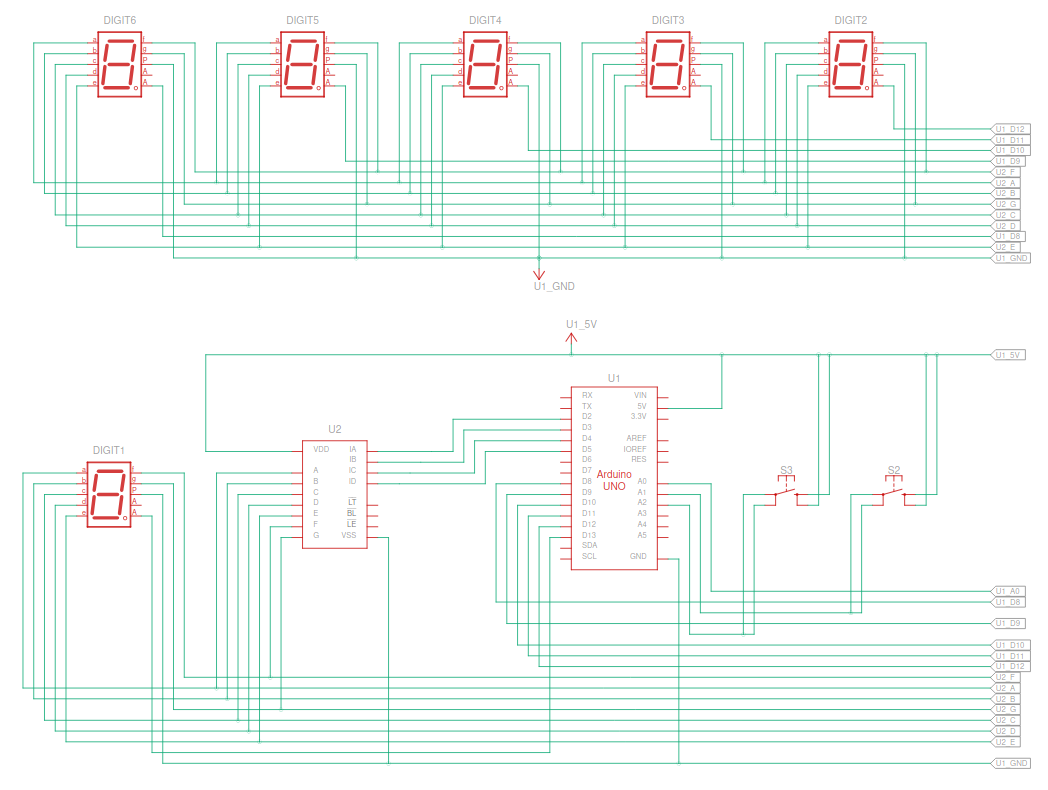
\includegraphics[width=0.6\linewidth]{figs/clp1.jpg}
    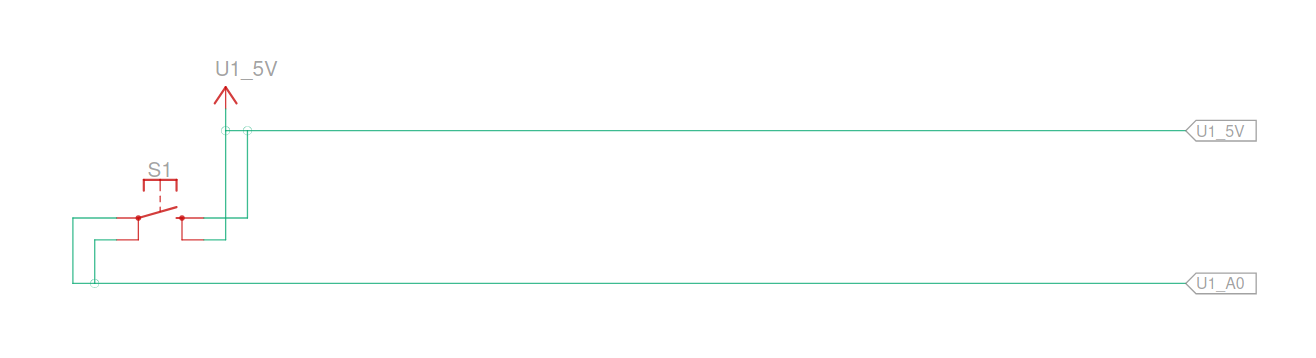
\includegraphics[width=0.6\linewidth]{figs/clp2.jpg}
    \caption{Circuit diagram}
    \label{fig:circ}
\end{figure}

The circuit diagram of the clock is given by fig. \ref{fig:circ}. There are six 7-segment displays(\texttt{DIGIT1} - \texttt{DIGIT6}), three buttons (\texttt{S1} - \texttt{S3}), one 7447 BCD to 7-Segment decoder, and one Arduino.

\begin{figure}
  \centering
  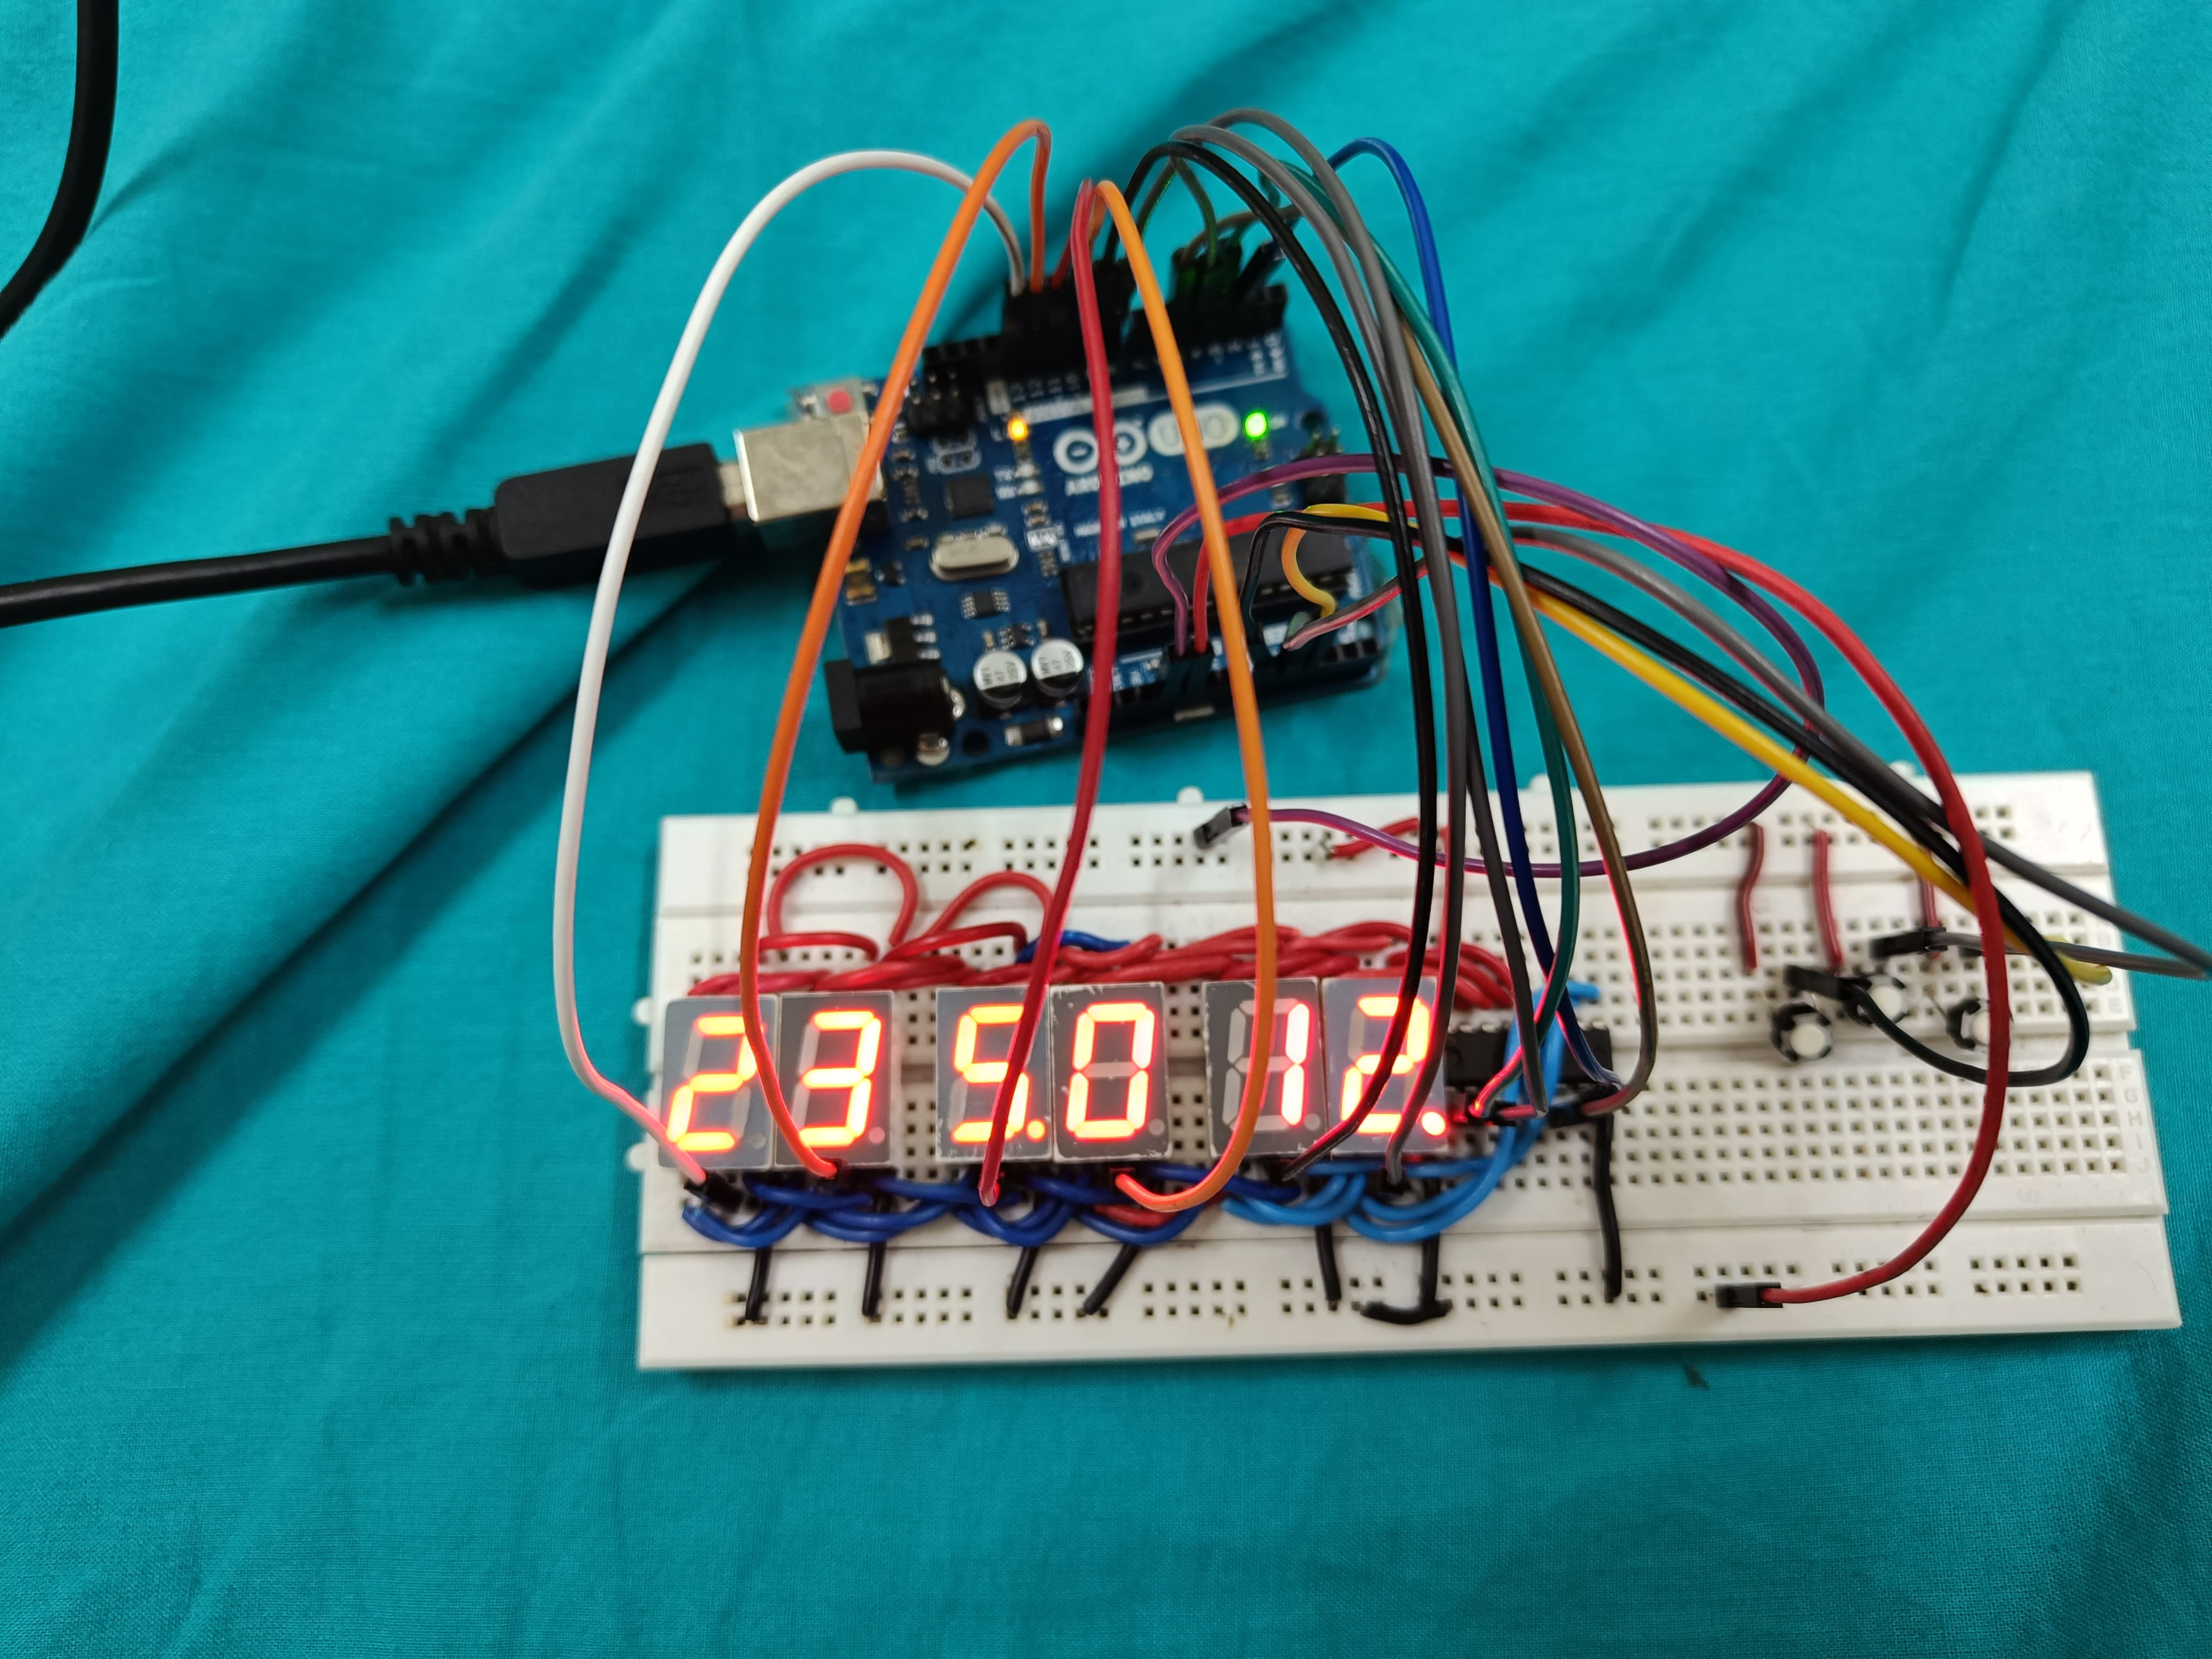
\includegraphics[width=1\linewidth]{figs/clkP.jpg}
  \caption{Physical Build}
\end{figure}

\section{Software Implementation}\label{section:sft}

% \lstinputlisting[style=avrc]{code/main.c}
The code for the driver:
\begin{lstlisting}
  ./code/main.c
\end{lstlisting}

The above code runs the clock. Like said before, we use the concept fo multiplexing. By that, I mean, I loop through each 7-segment display and power them for a short enough time (2ms). This will make it look like all the six of them are powered at the same time.

I have made three separate functions that increment hours, minutes and seconds separately and a nested if-else to join them all together. 

\section{User Interface}

The first mode is normal function mode, where it displays currently set time(\texttt{normal mode}). In mode two, we can set time being displayed(\texttt{set mode}).To switch between the modes, we press \texttt{S1}. 

Once you enter the \texttt{set mode}, the seconds segment will start blinking. This indicates currently seconds is selected to change. To circulate between seconds, minutes and hours segments, press \texttt{S}. The currently selected segment will blink. To change the time displayed the current segment, press \texttt{S3}. For hours and minutes, the time increments, meanwhile for seconds, it resets back to \texttt{00}. The clock doesn't stop ticking in this mode.

In \texttt{normal mode}, the clock runs normally and buttons \texttt{S2} and \texttt{S3} are disabled.

\section{Conclusion}

There are multiple improvements that can be done in the clock. First of all, the clock is not very accurate and looses a litte bit of time every day. Next thing that could be done is add an alarm system, making it further useful. As it is more of a clock and not a watch, we wouldn't need a stopwatch or a timer.

\end{document}
